\documentclass[11pt,a4paper]{article}
\usepackage{amsmath}
\usepackage{amsfonts}
\usepackage{amssymb}
\usepackage{graphicx}
\usepackage{fullpage}
\usepackage{hyperref}
\usepackage{tabulary}
\usepackage{amsthm}
\usepackage{syntax}
\usepackage{enumitem}
\usepackage{listings}
\usepackage{lipsum}
\usepackage{verbatim}
\usepackage{color}
\usepackage{mathtools}
\usepackage[left=2.5cm,right=2.5cm, top=2.2cm]{geometry}
\usepackage{graphicx}
\usepackage{caption}
\usepackage{subcaption}

\title{Final Report}
\author{Group 33\\Adela Baciu, Radu Gheorman\\ Nuri Cingillioglu, Kaiwen Song}
\date{June 2014}

\begin{document}

\maketitle

\section{Group Work, Organisation and Effectiveness}
During the earlier phase of the project, we took the approach of splitting the work so that everyone should gain experience with the C language, but also giving challenges to every member. The less experienced are given the utilities functions to gain style and familiarity with the language, while the more experienced ones deal with the debugging, designing and beautifying of code. We believe this approach was highly effective in achieving high efficiency, as everyone received work amount that was proportional to his/her abilities; it was also effective in making everyone feel valued, as everyone was able to accomplish a good deal during the early phase of the project. 

However, as the the group progressed to doing the extension, each member started cooperating a great deal more with each other, as it was something new for all of us and that by working as a group, we were able to make more progress. Such cooprerations include designing the circuits, research data-sheets and specifications in order to obtain information, and also writing codes as a group to prevent mistakes.

Throughout the project, we have maintained excellent communication. This is down to the way we worked, which we met up with every member of the group present on a regular basis, to discuss design and produce code. This particular approach ensured that everyone was up to date with the progress of everyone else, and that there would be no miscommunication between the members, thus ensuring good organisation and clarity. We have used other tools such as Trello to keep the tasks organised, and of course, Git, to enable everyone to be able to work on separate files at the same time to maintain productivity.

We really think the way that we planned the project: setting a design, dividing tasks and cooperation for every encountered problem (for example reading/printing binary files, utility functions for bit operations etc.), was effective. This is exemplified by the fact that we were able to finish the entire project in exactly one week after receiving the specification. And of course a lot of this is also down to the dedication displayed by every member of the group.

\section{Emulator - Short Description}

The emulator's pipeline consists of a fetch to a decode, execute cycle. The emulator executes the instruction immediately after it decodes the instruction. This design had a huge impact on the pipeline as our Program Counter points to the next instruction instead of the second next instruction as stated in the specification. We modified the behaviour of branching instructions to conform to this design explicitly, which seemed to be a sensible thing to do and which proved out to be very helpful towards finishing the tasks. 

The ARM structure is first initialized with GPIO taken into account then the binary file is read into the memory starting at position 0. The first instruction is fetched and then the Program Counter is increased after. When decoding, first the condition field is checked, if valid, then the type of the instruction is decoded to one of the four possibilities. Then, the 32-bit instruction and a pointer to the current ARM structure is passed to the respective instruction type decoder and executor which reside in different files. For example, if the instruction is a data processing instruction, it is passed into "dataprocessing.c" file, along with the pointer to the ARM structure, into an entry point function of the same name. It is decoded further, and executed immediately after updating the state of the ARM. 

Concluding, we didn't have any memory leaks, because we did not dynamically allocate memory, using only the stack.

\section{Assembler - Short Description}

The assembler had a similar pipeline design to the emulator. The design involved around a single main function inside "assemble.c" which orchestrated a \textbf{two pass} assembling process. There were 6 key steps that the main function did: read the text file, resolve labels, tokenise instructions, get hash code, decode and finally write to binary file. For each step, the main function called entry point functions in different files which performed the required tasks. The crucial point was that after each call, the program execution returned to the main function, maintaining an organised flow rather than jumping between random files during execution. All the files linked using a single header file "assemble.h", which included the most common libraries and avoided duplicate includes. Decoding instructions involved using a hash table for each instruction, and a corresponding function which returned the binary format of the instruction. Our hashing algorithm was a perfect hashing function for the given 23 instruction codes, giving an array of 25 elements with only 2 empty slots. 

One of the difficulties we had with the assembler was that there was a memory leak in "ldr rn, =" instruction which dynamically increased the memory to fit the 32 bit immediate value. We used valgrind to locate the source of the error and fix it. The expanded memory was not reported back to the main function which only freed the initial allocated memory but not the expanded part.

\section{LED Flashing}
On the same day when the Assembler’s tests were working, we started the 3rd part of the project, being the gpio program to flash the LEDs on the Pi. The implementation was straight forward, details are as follows: we started by setting the gpio 16 as the output pin and afterwards, clearing it. The next step was to create an infinite loop where we set the LED ON and OFF at an interval of roughly 1 second. To obtain the interval of time, we simply used a larger loop.

Fortunately, from the first try, our LED was beautifully flashing!

\newpage
\section{Extension}

\subsection{Choosing an Extension}
Deciding what we wanted to implement for our extension was definitely not an easy job. The very first idea for the extension was to make the Pi fly by using the GPIO pins to enable propellers attached onto the Pi. However, we have concluded that this approach was impossible due to the nature of flight mechanics, which a small time delay would result in unstable flights and crashes. Our second approach involving using the Raspberry Pi as a remote control to a drone with itself on board was also difficult due to the lack of PWM GPIO pins on the Pi.

After further discussion and research, the idea of using the Pi as a controller to lighting systems was put forward. As the group had prior experience in this field, we knew that this extension would be doable with the capabilities of the Pi. Hence this idea was chosen by us, knowing that it has the potential to amaze.

\subsection{Overall Description}

The industrial standard to controlling light systems involves using the DMX-512 protocol, which is a specified way of transmitting serial data. The protocol states that data are transmitted in DMX packet, which consists of padding around a byte of data, which is sent to devices connected in a serial fashion. A DMX packet consists of a break signal, which is a series of 0s, lasting minimum 88 microseconds, followed by 2 Mark after Break bits at 1, a start bit at 0, 8 bits data then 2 stop bits at 0.

The challenge for us was to use the Pi to simulate a controller that was able to generate outputs in this particular format. We needed to be able to read the data byte by byte from each memory allocation, adding the required padding to the data obtained, before finally outputting the data in a serial fashion. What was more challenging was the fact that we would have to do all of this in a timed fashion, as the protocol only accepts signals of valid time frames. This meant that we had to find a way to output serial data at the speed which we state to the Pi. 

We used our own assembler as the operating system for the Pi, by writing an entire assembly file consisting of instructions, stating the behaviours of the Pi. In the assembly file, the output pin was set then cleared, and we manually written data into memory addressed and polled from it. If our design works, then hopefully these instructions would enable the GPIO pins stated in the file to be outputting serial, industrial standard data.

\subsection{Testing}

\subsubsection{USB DMX Reader}
Luckily, we had a reliable method that we could use to test our implementations. We had access to a DMX controller, which was an industrial standard device, which when supplied with serial data stream, along with its negated stream, which we will refer to as data minus, and a ground, was able to determine the validity and the contents of the signal transmitted, with the aid of an accompanying software. This device was also helpful in the respect that it was able to give us industrial standard outputs when specified with data, hence we could use such outputs to compare against our own to debug.

The DMX Reader is the software accompanied the DMX controller. Through the DMX Reader we are able to read in the inputs from the Pi and display it on a computer. If everything works, the DMX Reader will be able to decode the serial input stream and obtain the data transferred to it by removing the padding and display the decimal number represented by the 8 bits data. 
\subsubsection{Oscilloscope}
The DMX Reader and controller enabled us to test whether our design was able to output industrial standard data, however, if the format of our output was wrong, then testing it on the DMX will only produce junk data outputs that did not help us. So we wanted to find a remote and portable way to test our output. Under the suggestion of the CSG, we obtained ourselves a working oscilloscope. The idea behind the oscilloscope was that it was able to output visual representation of the data being transmitted by the pins. The oscilloscope helped us to analyse the data signal, to ensure that we had all the padding bits surrounding the data bits, and also to check our timing against the standard outputted by the DMX controller by reading the wavelength of outputs of the Pi.


\subsection{Implementation}

\subsubsection{Manually turning on and off the pins}
The initial naive attempt at outputting a DMX signal was to manually turn on and off GPIO pins, as it would have been quite similar to flashing a LED. However, this approach bared significant problems, one of which was \textbf{timing}. After trying a few times to turn on and off the pins 14 and 15 to simulate data plus and data minus, we realized it was impossible to achieve 4 microsecond precision using this method.

\subsubsection{Enabled the UART to output data}
Going over the Broadcom Peripherals spec, we discovered that there was a built-in serial output function, \textbf{UART} at GPIO pin 14. Though the specification was quite vague on how to the use this function, we managed to output the 8-bit data with 1 start bit and 2 stop bits. However, again the timing was off and the DMX protocol required a \textbf{break}.

\subsubsection{Using an inverter to simulate the data}
After confirming that we were outputting the correct data using an oscilloscope, we tried to simulate data minus as the standard on which DMX is based, RS-485, uses \textbf{differential signalling}. After double checking that the UART inside the Broadcom 2835 chip only provided a single output without any built-in data minus option, we sought an \textbf{inverter} to invert the signal. Our concern was if the delay of the inverter would corrupt the data that was being sent from the original data plus line. Fortunately, the delay was negligible.

\subsubsection{Simulating break manually by disabling pin 14}
One of the most challenging part of outputting a valid DMX signal was simulating the break. The UART of the Pi outputted logical high when on idle and then the data. However, the protocol required a low signal for more than 88 microseconds to signal the packet. Our initial attempt was to turn off the GPIO output pin such that it will run low for some period of time and then turn back on to output the data. The idea failed quickly as we realised that the pin was dependant on the UART and continued to output high.

\newpage
\subsubsection{Using the multiplexer to simulate breaks}
In this attempt to simulate the break, we incorporated a\textbf{multiplexer} to flip the signals of idle and output low for a period of time. We used GPIO 8 as a control signal to the multiplexer. However, the multiplexer did not behave as expect it to be, introducing delays when switching between signals. The multiplexer together with the GPIO 8 made timing 88 microseconds incredibly difficult.

\subsubsection{Cross referencing with the original output of the DMX}
Our biggest progress happened when we analysed a proper DMX signal from the USB-DMX device using our oscilloscope. We noticed several crucial points first of which was that our timing with the current baud rate was not at 4 microseconds and that the oscilloscope \textbf{had not been calibrated}. The initial UART clock of the Pi was at 3 MHz which was insufficient to output DMX. Furthermore, we discovered that the \textbf{break was not visible} in the oscilloscope.

\subsubsection{Setting the UART clock and slow down the baud rate to simulate break}
We manually increased the UART clock to 4 MHz which gave an exact baud rate of 250k required by the DMX protocol. We confirmed this by checking out bit lengths in the oscilloscope with respect to the proper output we recorded in the previous step. Since we had control of the output speed, we simulated the break by \textbf{slowing} the baud rate and outputting data 0 from UART. The slowing down ratio was 2.5 to fit the 8-bit data, 1 start bit, 2 stop bits in the range of 88 to 176 microseconds. This method not only outputted consistent breaks, but also maintained a smooth stream of data as the UART was not manually turned off.

\subsection{Final Product}
Our final product involved an assembly program which was able to output data stored as binary inside the kernel image itself. The output data is divided into scenes which usually described what each light should do. We put this data inside a text file and wrote a helper program which converted into a binary file. Then we wrote another helper program which concatenated the assembly program binary and the data binary such that the assembly program would access the data from the memory locations. There was a slight problem as we were not able to access the memory locations of the data directly as we thought the kernel image started at address 0x0. It turned out the kernel image start address was 0x8000 (which we had to search for online). After resolving addressing issues, the final assembly program was able to output a set of data, defined as a scene, for a certain amount of delay specified inside the show file and then move onto the next scene looping forever.

\section{Individual Reflections}

\subsection{Adela:}
From my point of view, I honestly think the decision of: firstly agree on a design, splitting the work and then join whenever it was needed, was best for us as a group, since each member had to learn from this project, on his/her own (not in a selfish way, but in a way so that everyone would gain confidence with the C language and experience in debugging and fast quality coding). 
      I thought one of my strengths will be the C++ experience and proved right, opposite to the leak, which I really thought it will be the tiredness, but instead was the lack of resistance and the inability of focus after more than 5 hours. 
      
\subsection{Radu:}
To begin with, I am sure that I took part in a group of teammates, and that's the main key of our story for this project. We helped each others as much as we could, we spent a lot of time focusing on getting everyone aware of what we would be doing, we made sure that the design we had is the result of everyone's contribution. Moreover, I guess everyone’s experience of working in a group was broadened with this project, and perhaps not only the working in a group experience, but the C programming skills as well. For me, this was by far the best experience of programming in a group, and this is thanks to all my team mates who've made working in a group so enjoyable.

\subsection{Nuri:}
In my opinion, the group was quite balanced such that there were tasks for everyone’s respective level of programming experience and knowledge. I think the project benefitted the other group members to improve their skills in C and understanding of low level interactions such as memory management. Though, it took some time for other group members to adjust to C after programming in Java, they started to appreciate the power it provides. Unlike a goal oriented agile development imposed in tutorials and exams, the project highlighted to the group members the craftsmanship of programming.


\subsection{Kaiwen:}
In many aspects, this project has been an eye-opener for me. This was one of the first times where I had not taken up a main role when working as a group, and I often had to keep up with my teammates. A lack of programming experience meant that I was fearful at first to approach the task, knowing I will likely to slow the group down during the programming phase. Luckily, from experience, the team knew the right approach to the project. By dividing up the tasks, I was eased into the whole thing by first working on the less demanding codes, then gradually working my way up.

As I feared, I was not as productive as other members of the group during the programming phase. However, my group has done an excellent job at helping me to become more involved in the task by sharing the task or programming together. I definitely have gained more confidence as the project progressed. By the end, I was somewhat regretting that I had not been more proactive in claiming tasks to do, which is definitely a sign of progress that has been made.

Overall, I believe we had the right balance between professionalism, productivity and fun. I did not know two of the guys in the group before the project but by the end we became good friends; and although we worked hard throughout the task, it never felt boring or tedious. I think the key to our success was that we never blamed, but helped instead, when someone makes a mistake; and when we got stuck doing the extension, the team did not give up and carried on. I have gotten a lot more than just programming experience out of this project, and that is full credits to the team, they have been a pleasure to work with.


\newpage


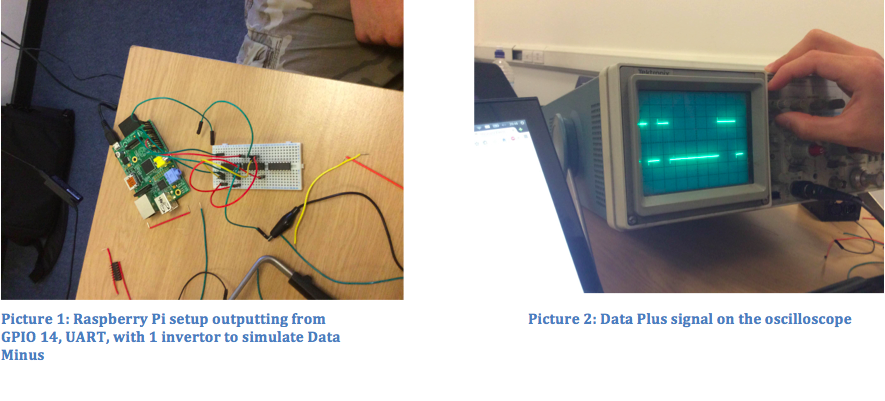
\includegraphics[width=1\linewidth]{images/photo1}

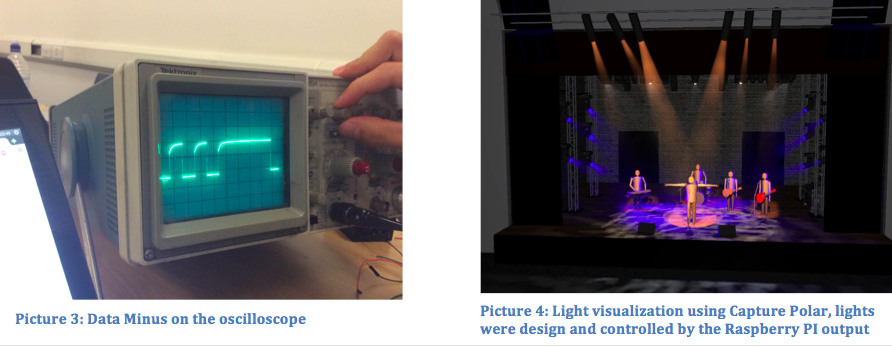
\includegraphics[width=1\linewidth]{images/photo2} 



\end{document}







